\chapter{什么是呼吸作用？}\label{ch:g7:what-is-respiration}

把一只潮虫放入密闭的罐子中，几小时后，罐中的空气
已经发生变化：其中的\omterm{def:g7:what-is-respiration:respiration}{氧气}减少了，代之以
\omterm{def:g7:what-is-respiration:respiration}{二氧化碳}。换成\omterm{def:g2:from-seed-to-plant:germination}{萌发}的\omterm{def:g2:from-seed-to-plant:seed}{种子}、一朵蘑菇、一条
金鱼、一勺活\omterm{def:g6:decomposers-and-soil:soil}{土壤}——结果相同，
每次皆然。\Cref{prop:g4:breathing:exchange}已在
你自己的胸腔中展示了这种交换；本年将这一观点拓展至完整的广度：
这种交换并非人类的习惯，而是生命本身的属性。

\section{呼吸作用的定义与测量}

\begin{definition}[呼吸作用]\label{def:g7:what-is-respiration:respiration}
\emph{呼吸作用}\index{呼吸作用}是一种气体交换，\omterm{def:g6:exploring-our-environment:components}{生物}借此
由此从周围\omterm{def:g6:exploring-our-environment:components}{环境}中摄取\emph{氧气}\index{氧气}，
并释放\emph{二氧化碳}\index{二氧化碳}。
它不可与
\emph{呼吸}\index{呼吸}相混淆——即可见的胸部
运动（见\cref{def:g4:breathing:movements}）：呼吸是
\emph{实现}呼吸作用的一种方式；
呼吸作用本身则是气体交换，它在每个活\omterm{def:g5:first-look-at-cells:cell}{细胞}中持续进行，
无论是否伴有运动。
\end{definition}

\begin{proposition}[如何显示气体交换]\label{prop:g7:what-is-respiration:shown}
两个\omterm{def:g3:sorting-living-things:criterion}{标准}的实验室检测可以揭示\omterm{def:g7:what-is-respiration:respiration}{呼吸作用}：
\begin{itemize}
  \item 将\emph{\omterm{def:g7:what-is-respiration:respiration}{氧气}探头}放入密闭容器中，显示
        \omterm{def:g6:exploring-our-environment:components}{生物}置于其中时，\omterm{def:g7:what-is-respiration:respiration}{氧气}含量
        下降；
  \item \emph{澄清石灰水}\index{澄清石灰水}，一种透明液体，
        遇\omterm{def:g7:what-is-respiration:respiration}{二氧化碳}会变浑浊；把容器内的空气通入其中时，
        它也会变浑浊。
\end{itemize}
\omterm{def:g7:what-is-respiration:respiration}{氧气}下降、\omterm{prop:g7:what-is-respiration:shown}{澄清石灰水}变浑浊，而无生命的
对照容器保持不变，
（见\cref{met:g4:what-plants-need:fairtest}——公平实验
处处相随）：这就是经过测量的\omterm{def:g7:what-is-respiration:respiration}{呼吸作用}。
\end{proposition}
\admitted

\begin{example}[呼吸者展览]\label{ex:g7:what-is-respiration:gallery}
对一批\omterm{def:g6:exploring-our-environment:components}{生物}进行这两项测试：小鼠——\omterm{def:g7:what-is-respiration:respiration}{氧气}迅速下降，
石灰水很快变浑浊；潮虫——情况相同，个头更小；\omterm{def:g2:from-seed-to-plant:germination}{萌发}的豌豆
——结果一目了然（一罐发芽的豌豆
一天之内即可耗尽其\omterm{def:g7:what-is-respiration:respiration}{氧气}）；蘑菇——有；池塘
螺——有；一勺活\omterm{def:g6:decomposers-and-soil:soil}{土壤}——有，其中
数十亿\omterm{def:g6:decomposers-and-soil:decomposers}{分解者}共同进行\omterm{def:g7:what-is-respiration:respiration}{呼吸作用}
（见\cref{ex:g6:decomposers-and-soil:handful}）。只有
对照罐——装有卵石、干沙——毫无变化。
\end{example}

\begin{omfigure}
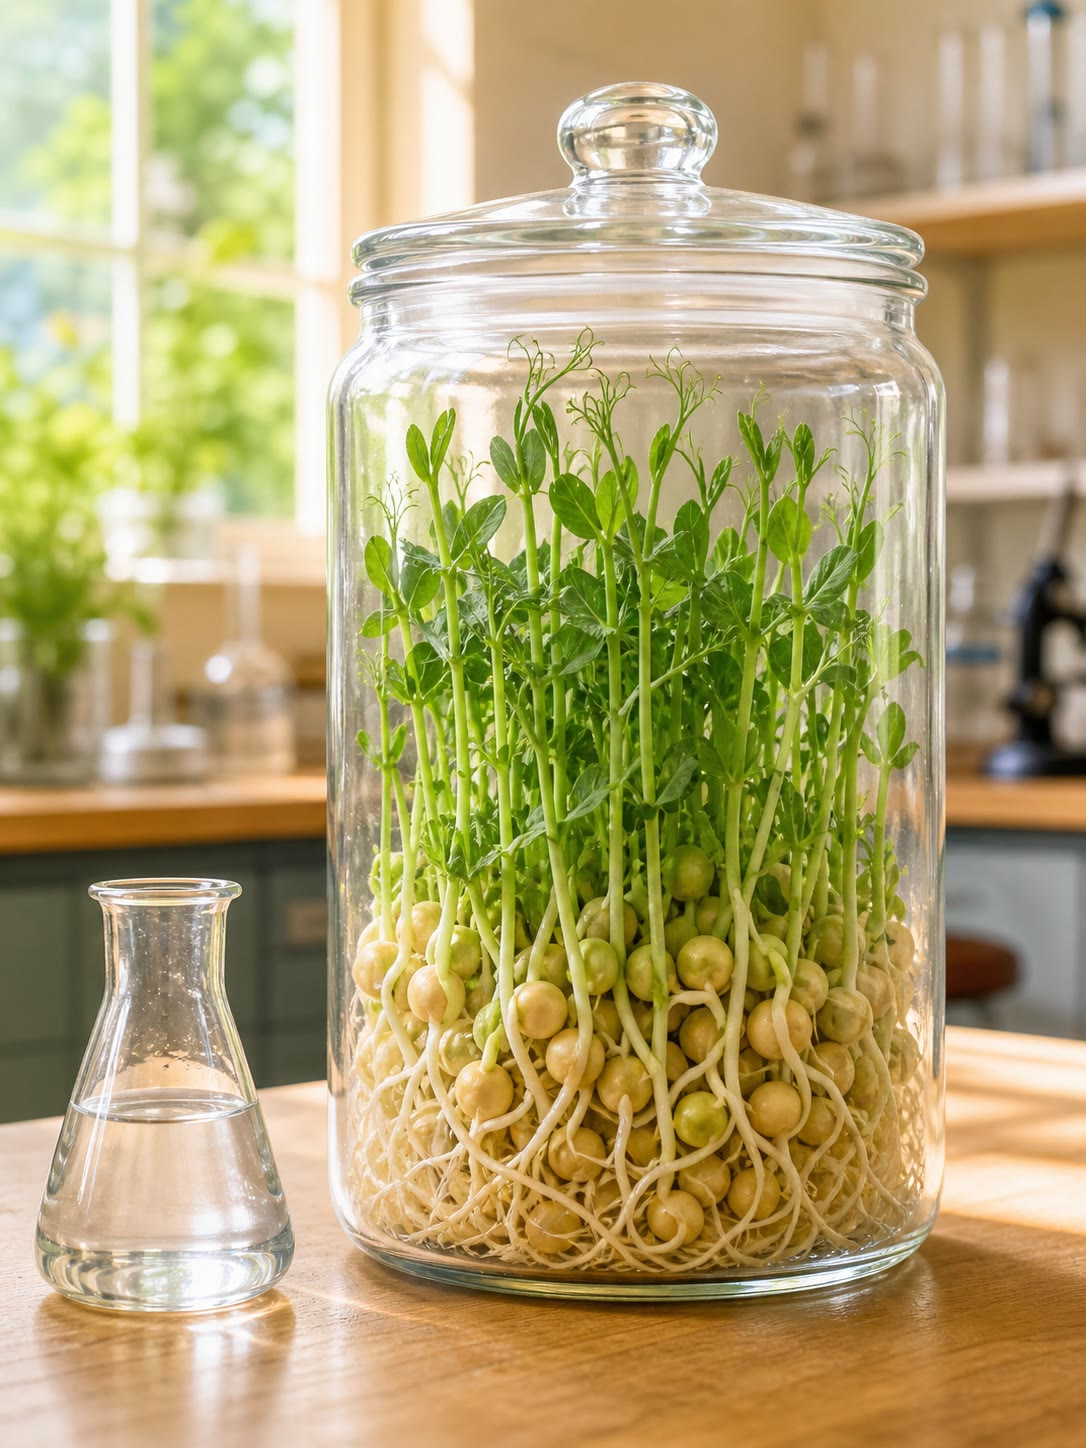
\includegraphics[width=0.46\linewidth]{images/book1/ai/g7-resp-peajar.jpg}

{\small 实验台上最不起眼的\omterm{def:g7:what-is-respiration:respiration}{呼吸}者：一罐
\omterm{def:g2:from-seed-to-plant:germination}{萌发}的豌豆，一天之内即可耗尽\omterm{def:g7:what-is-respiration:respiration}{氧气}。}
\end{omfigure}

\begin{remark}[植物同样进行呼吸]\label{rem:g7:what-is-respiration:plants}
\Cref{rem:g6:plants-are-producers:gas}曾顺带提到此事；
罐中的实验证明了这一点：盆栽\omterm{def:g1:plants-around-us:plant}{植物}\emph{在黑暗中}
使其罐中\omterm{def:g7:what-is-respiration:respiration}{氧气}减少，使\omterm{prop:g7:what-is-respiration:shown}{澄清石灰水}变浑浊，与任何\omterm{def:g1:animals-around-us:animal}{动物}相同。在
白天，\omterm{def:g5:food-webs:roles}{生产者}的制造作用掩盖了这一效应——
吸收的\omterm{def:g7:what-is-respiration:respiration}{二氧化碳}远多于\omterm{def:g7:what-is-respiration:respiration}{呼吸作用}释放的量
——但\omterm{def:g7:what-is-respiration:respiration}{呼吸作用}从未停止。绿色并不能让
\omterm{def:g5:first-look-at-cells:cell}{细胞}免除广义上的\omterm{def:g7:what-is-respiration:respiration}{呼吸}；没有任何\omterm{def:g6:exploring-our-environment:components}{生物}可以
例外。
\end{remark}

\section{生物为何进行呼吸作用}

\begin{proposition}[呼吸作用为细胞提供动力]\label{prop:g7:what-is-respiration:power}
气体交换的意义在于\emph{\omterm{prop:g3:balanced-diet:jobs}{能量}}。在每个活\omterm{def:g5:first-look-at-cells:cell}{细胞}中，
\omterm{def:g4:journey-of-food:digestion}{营养物质}（见\cref{def:g4:journey-of-food:digestion}）
被\omterm{def:g7:what-is-respiration:respiration}{呼吸作用}带来的\omterm{def:g7:what-is-respiration:respiration}{氧气}缓慢地\emph{燃烧}：
其\omterm{prop:g3:balanced-diet:jobs}{能量}被释放，供\omterm{def:g5:first-look-at-cells:cell}{细胞}做功——
收缩、建造与调控——而\omterm{def:g7:what-is-respiration:respiration}{二氧化碳}是燃尽后的残留物，
被运走。
\Cref{prop:g6:matter-from-food:losses}中的“被燃烧的部分”
正是此事，只是从账本角度看；此处则
从\omterm{def:g5:first-look-at-cells:cell}{细胞}的角度来看。
\end{proposition}
\admitted

\begin{example}[如实使用的火焰类比]\label{ex:g7:what-is-respiration:fire}
蜡烛火焰同样消耗\omterm{def:g7:what-is-respiration:respiration}{氧气}并释放
\omterm{def:g7:what-is-respiration:respiration}{二氧化碳}——燃烧与\omterm{def:g7:what-is-respiration:respiration}{呼吸作用}确实是同类
化学过程。两者的差异同样重要：
\omterm{def:g5:first-look-at-cells:cell}{细胞}内的燃烧缓慢、无焰，分散在数千个
微小步骤中，其\omterm{prop:g3:balanced-diet:jobs}{能量}被用于做功，而非
以光和灼热的形式散失。\omterm{def:g7:what-is-respiration:respiration}{呼吸作用}是
被驯化的燃烧——拴着缰绳的火，存在于你体内的每个\omterm{def:g5:first-look-at-cells:cell}{细胞}中。
\end{example}

\begin{example}[解读呼吸需求]\label{ex:g7:what-is-respiration:demand}
由于燃烧为工作提供动力，需求随努力程度而变化：
\cref{ex:g4:breathing:running}中那个冲刺的孩子
\omterm{def:g7:what-is-respiration:respiration}{呼吸}远比坐在扶手椅上的读者快得多；
\omterm{def:g2:from-seed-to-plant:germination}{萌发}的豌豆——全速构建植株
（见\cref{def:g2:from-seed-to-plant:germination}）——其\omterm{def:g7:what-is-respiration:respiration}{呼吸}
远快于旁边干燥、静止等待的\omterm{def:g2:from-seed-to-plant:seed}{种子}，后者的
\omterm{def:g7:what-is-respiration:respiration}{呼吸}几近于零，可持续数年。\omterm{def:g7:what-is-respiration:respiration}{呼吸作用}是
生命的“引擎轰鸣”：用力和生长时响亮，
休眠时细若低语，只有死亡才会使其沉寂。
\end{example}

\section{各类栖息地中的呼吸作用}

\begin{proposition}[需求相同，环境各异]\label{prop:g7:what-is-respiration:habitats}
所有\omterm{def:g6:exploring-our-environment:components}{生物}都必须\emph{从周围
\omterm{def:g6:exploring-our-environment:components}{环境}}中获取\omterm{def:g7:what-is-respiration:respiration}{氧气}——而\omterm{def:g6:exploring-our-environment:components}{环境}各不相同。空气
富含\omterm{def:g7:what-is-respiration:respiration}{氧气}；水中溶解的\omterm{def:g7:what-is-respiration:respiration}{氧气}要少得多，
（\cref{exo:g4:breathing:11}已涉及这一后果）；\omterm{def:g6:decomposers-and-soil:soil}{土壤}和
淤泥中的\omterm{def:g7:what-is-respiration:respiration}{氧气}则更少。\omterm{def:g6:exploring-our-environment:components}{生物}在何处生活、如何生活，
因此取决于它如何解决\omterm{def:g7:what-is-respiration:respiration}{氧气}问题——
接下来两章的主题：\omterm{def:g1:animals-around-us:animal}{动物}的
\omterm{def:g7:what-is-respiration:respiration}{呼吸}装备（见\cref{ch:g7:how-animals-breathe}）与
水\omterm{def:g6:exploring-our-environment:components}{环境}中的供氧状况（见\cref{ch:g7:oxygen-in-the-water}）。
\end{proposition}
\admitted

\begin{method}[测试一个关于呼吸作用的问题]\label{met:g7:what-is-respiration:test}
为检验任何关于\omterm{def:g7:what-is-respiration:respiration}{呼吸作用}的论断（“\omterm{def:g2:from-seed-to-plant:seed}{种子}在温暖时\omterm{def:g7:what-is-respiration:respiration}{呼吸}更快”、
“池塘淤泥会\omterm{def:g7:what-is-respiration:respiration}{呼吸}”）：
\begin{enumerate}
  \item 将研究对象封入容器，并配置\omterm{def:g7:what-is-respiration:respiration}{氧气}探头
        或\omterm{prop:g7:what-is-respiration:shown}{澄清石灰水}陷阱；
  \item 设置孪生对照——容器相同，
        但研究对象缺席或已死亡；
  \item 若论断指明了某一\omterm{def:g6:exploring-our-environment:conditions}{条件}，则每次只改变一个\omterm{def:g6:exploring-our-environment:conditions}{条件}
        （\omterm{def:g6:exploring-our-environment:conditions}{温度}、\omterm{def:g6:exploring-our-environment:conditions}{湿度}或黑暗）；
  \item 由差异读出结论：\omterm{def:g7:what-is-respiration:respiration}{氧气}减少、
        石灰水变浑浊——与对照的静止相比；
        对照则无任何变化。
\end{enumerate}
\end{method}

\begin{example}[对低温种子应用该方法]\label{ex:g7:what-is-respiration:coldseed}
论断：正在\omterm{def:g2:from-seed-to-plant:germination}{萌发}的豌豆在低温下\omterm{def:g7:what-is-respiration:respiration}{呼吸}得更慢。
取两瓶发芽的豌豆，一瓶置于室温，一瓶放入
冰箱；两瓶均设\omterm{prop:g7:what-is-respiration:shown}{澄清石灰水}陷阱；另取第三瓶已死亡的豌豆作为对照。
次日：温暖瓶中的石灰水变浑浊，
低温瓶中仅微微起雾，对照瓶保持澄清。结论：
\omterm{def:g7:what-is-respiration:respiration}{呼吸作用}的强弱与豌豆的活动速度一致——
即\cref{prop:g6:decomposers-and-soil:speed}中的
\omterm{def:g6:exploring-our-environment:conditions}{条件}规律，只是以气体来测量。
\end{example}

\section{练习}

\begin{exercise}[$\star$]\label{exo:g7:what-is-respiration:1}
定义\omterm{def:g7:what-is-respiration:respiration}{呼吸作用}，并区分它与\omterm{def:g7:what-is-respiration:respiration}{呼吸}。
\end{exercise}

\begin{exercise}[$\star$]\label{exo:g7:what-is-respiration:2}
说出能揭示\omterm{def:g7:what-is-respiration:respiration}{呼吸作用}的两种实验台检验方法，
并说明各自显示的内容。
\end{exercise}

\begin{exercise}[$\star$]\label{exo:g7:what-is-respiration:3}
为什么每一个\omterm{def:g7:what-is-respiration:respiration}{呼吸作用}实验都需要一个已死亡的
对照容器？
\end{exercise}

\begin{exercise}[$\star$]\label{exo:g7:what-is-respiration:4}
\omterm{def:g7:what-is-respiration:respiration}{呼吸作用}有何意义，依据
\cref{prop:g7:what-is-respiration:power}？按此，
\omterm{def:g7:what-is-respiration:respiration}{二氧化碳}又是什么？
\end{exercise}

\begin{exercise}[$\star$]\label{exo:g7:what-is-respiration:5}
列出五种差异很大的\omterm{def:g6:exploring-our-environment:components}{生物}，它们在
\cref{ex:g7:what-is-respiration:gallery}中均展示了\omterm{def:g7:what-is-respiration:respiration}{呼吸作用}。
\end{exercise}

\begin{exercise}[$\star$]\label{exo:g7:what-is-respiration:6}
白天的光照会掩盖其效应，
那么如何证明\omterm{def:g1:plants-around-us:plant}{植物}也在进行\omterm{def:g7:what-is-respiration:respiration}{呼吸作用}？
\end{exercise}

\begin{exercise}[$\star\star$]\label{exo:g7:what-is-respiration:7}
请给出蜡烛燃烧与\omterm{def:g5:first-look-at-cells:cell}{细胞}\omterm{def:g7:what-is-respiration:respiration}{呼吸作用}之间
两个确实相似之处与两个确实不同之处。
\end{exercise}

\begin{exercise}[$\star\star$]\label{exo:g7:what-is-respiration:8}
按\omterm{def:g7:what-is-respiration:respiration}{呼吸}速率排序，并说明理由：干燥的豌豆、
正在\omterm{def:g2:from-seed-to-plant:germination}{萌发}的豌豆、正在短跑的儿童、正在阅读的儿童。
\end{exercise}

\begin{exercise}[$\star\star$]\label{exo:g7:what-is-respiration:9}
一个密封瓶中装有正在发芽的豌豆，放置一夜；
次日早晨放入一支蜡烛，蜡烛立即熄灭。
请结合本章内容加以解释，
并说明与此同时\omterm{prop:g7:what-is-respiration:shown}{澄清石灰水}陷阱会显示什么。
\end{exercise}

\begin{exercise}[$\star\star$]\label{exo:g7:what-is-respiration:10}
依据\cref{met:g7:what-is-respiration:test}，设计
验证“活\omterm{def:g6:decomposers-and-soil:soil}{土壤}会进行\omterm{def:g7:what-is-respiration:respiration}{呼吸作用}；
经烘烤、已死亡的\omterm{def:g6:decomposers-and-soil:soil}{土壤}不会。”的实验。
\end{exercise}

\begin{exercise}[$\star\star$]\label{exo:g7:what-is-respiration:11}
为什么粮仓管理员担心潮湿的谷物堆
会自行升温？请结合
\cref{ex:g7:what-is-respiration:demand}与堆肥堆的
\omterm{def:g6:exploring-our-environment:conditions}{温度}
（\cref{ex:g6:decomposers-and-soil:compost}）加以说明。
\end{exercise}

\begin{exercise}[$\star\star\star$]\label{exo:g7:what-is-respiration:12}
“\omterm{def:g7:what-is-respiration:respiration}{呼吸}是行为，\omterm{def:g7:what-is-respiration:respiration}{呼吸作用}是化学过程；前者服务于后者。”
请为每一分句各用一项观察结果加以论证，
观察结果取自本章或
\cref{ch:g4:breathing}。
\end{exercise}

\section{问题：密封的瓶子}

\begin{problem}[{周末问题——六个瓶子，两个谜团，
一次气体交换}]\label{pb:g7:what-is-respiration:1}
为准备科学展览，班级准备了六个密封瓶，
每瓶均配有\omterm{def:g7:what-is-respiration:respiration}{氧气}探头和\omterm{prop:g7:what-is-respiration:shown}{澄清石灰水}陷阱：A——
卵石；B——干燥的豌豆；C——正在\omterm{def:g2:from-seed-to-plant:germination}{萌发}的豌豆；D——
一只小鼠（备有食物和水，且仅在教师看护下停留数小时）；
E——置于光照下的绿色\omterm{def:g1:plants-around-us:plant}{植物}；F——
置于暗箱中的同种\omterm{def:g1:plants-around-us:plant}{植物}。

\medskip\noindent\textbf{第一部分——预测。}
\begin{enumerate}
  \item 预测 A 瓶的读数，并说明
        A 瓶在实验中的作用。
  \item 预测 B 瓶与 C 瓶，并解释二者的差异，
        尽管两瓶中装的都是“同样的”豌豆。
  \item 预测 D 瓶的结果，并说明教师为何限制
        停留的时长。
  \item E 瓶与 F 瓶中的\omterm{def:g1:plants-around-us:plant}{植物}完全相同。预测每瓶中
        \omterm{def:g7:what-is-respiration:respiration}{氧气}的变化趋势，并利用
        \cref{rem:g7:what-is-respiration:plants}调和两者的差异。
\end{enumerate}

\medskip\noindent\textbf{第二部分——结果与读数。}
\begin{enumerate}[resume]
  \item 上午的数据与预测相符，但
        有位同学惊讶于 F 瓶中的\omterm{def:g1:plants-around-us:plant}{植物}“像\omterm{def:g1:animals-around-us:animal}{动物}一样\omterm{def:g7:what-is-respiration:respiration}{呼吸}”。
        请说明 F 瓶实际显示了什么，
        以及 E 瓶掩盖了什么。
  \item C 瓶的\omterm{def:g7:what-is-respiration:respiration}{氧气}每克豌豆的下降速度，
        是 B 瓶的三倍。请用
        \cref{ex:g7:what-is-respiration:demand}的术语来解释这一三倍的因子。
  \item D 瓶的石灰水变浑浊得最快。请用四步
        说明从小鼠温暖、活动的身体
        到乳白色液体之间的链条。
  \item 请用一句以
        “每一种\omterm{def:g6:exploring-our-environment:components}{生物}……”开头的话，
        写出 B、C、D、F 瓶共同支持的唯一结论。
\end{enumerate}

\medskip\noindent\textbf{第三部分——深入探究。}
\begin{enumerate}[resume]
  \item 提议加入第七个瓶子，内装蘑菇切片。预测
        其读数，并说明它会补充
        \cref{ex:g7:what-is-respiration:gallery}
        中哪一个界一级的要点。
  \item 展会参观者问：C 瓶对农民为何重要？
        请以
        \cref{exo:g7:what-is-respiration:11}中的粮仓为例作答。
  \item 第八个瓶子：带淤泥的池塘水。夜间
        \omterm{def:g7:what-is-respiration:respiration}{氧气}下降。瓶中哪些\omterm{def:g6:exploring-our-environment:components}{生物}正在进行\omterm{def:g7:what-is-respiration:respiration}{呼吸作用}，
        这一发现对\cref{ch:g7:oxygen-in-the-water}
        中提出的问题有何意义？
  \item 请以本章的区分作为展会海报的结尾：
        哪些瓶子显示了\emph{\omterm{def:g7:what-is-respiration:respiration}{呼吸}}，
        哪些瓶子显示了\emph{\omterm{def:g7:what-is-respiration:respiration}{呼吸作用}}？（注意——
        同一个词涵盖了它们全部。）
\end{enumerate}
\end{problem}
